\documentclass{article}
\usepackage{graphicx} % Required for inserting images
\usepackage{amsmath}
\usepackage{amssymb}
\usepackage{indentfirst}
\usepackage{float}
\usepackage[a4paper, total={6in, 10in}]{geometry}

\title{Mathcamp 2026 Qualifying Quiz Problem 2 Solution}
\author{Applicant ID: 25107}
\date{}

\begin{document}
	
	\maketitle
	
	We claim that the maximum roundness of a figure is $\frac{3}{\pi}$. Notice that each pentabend has 2 `concave' arcs and 3 `convex' arcs, shown in red and blue below respectively. \\
\begin{figure}[h]
    \centering
    \vspace{-0.3cm}
    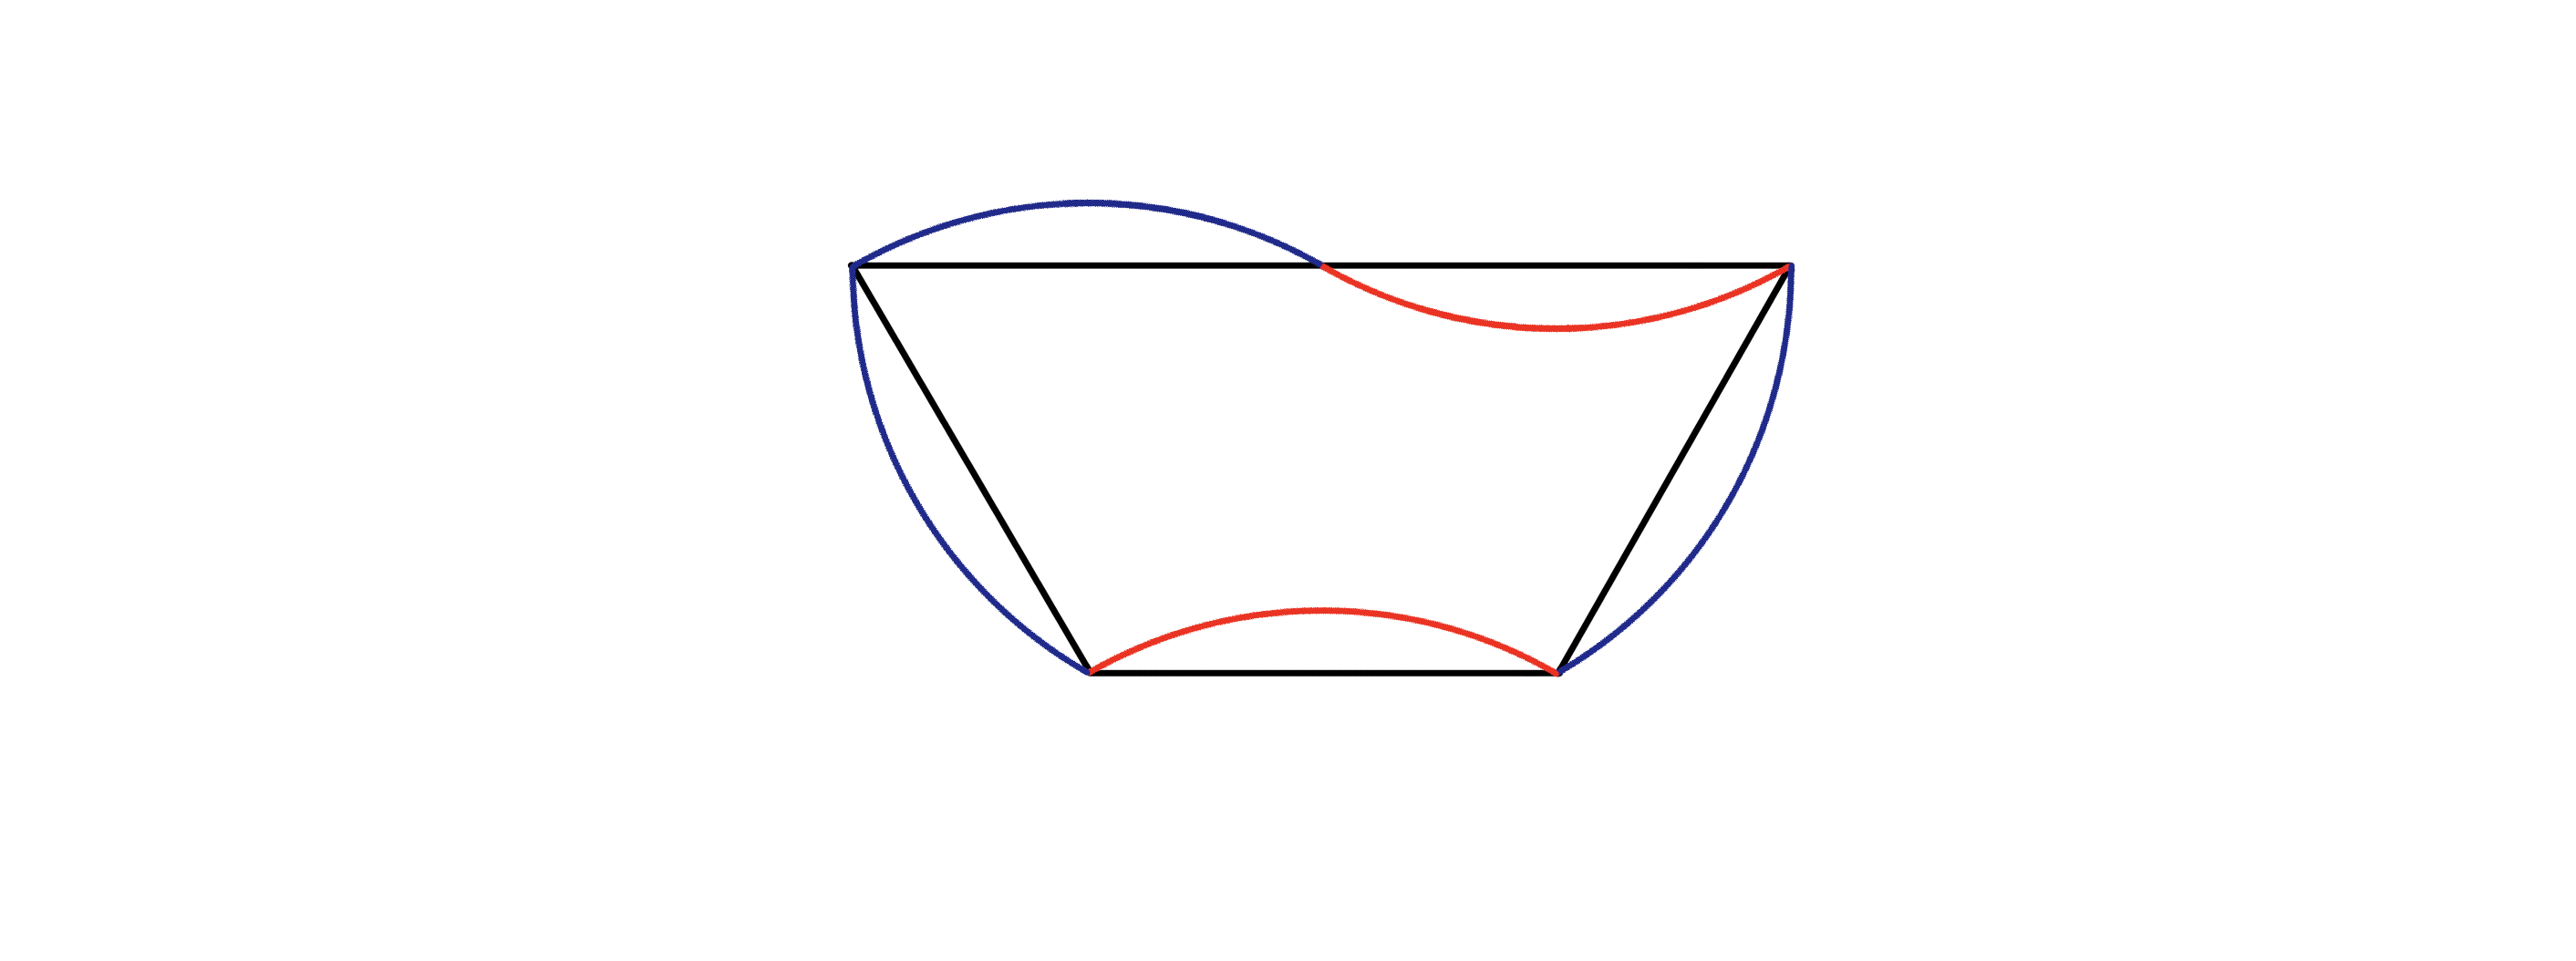
\includegraphics[width=10cm, trim = 5cm 3cm 5cm 2cm, clip]{convexity.png}
    \vspace{-0.3cm}
\end{figure}

    All joins must consist of a convex and a concave arc joining together, so the number of convex and concave arcs that are part of joins is equal. To maximize the roundness, we must minimize the perimeter that each pentabend will contribute to the shape. To do this, we have to maximize the number of joined arcs, and at best the joins will use 2 concave and 2 convex arcs from each pentabend, using up all the convex arcs. This is achievable in the infinite tiling below:\\
\begin{figure}[h]
    \centering
    \vspace{-0.3cm}
    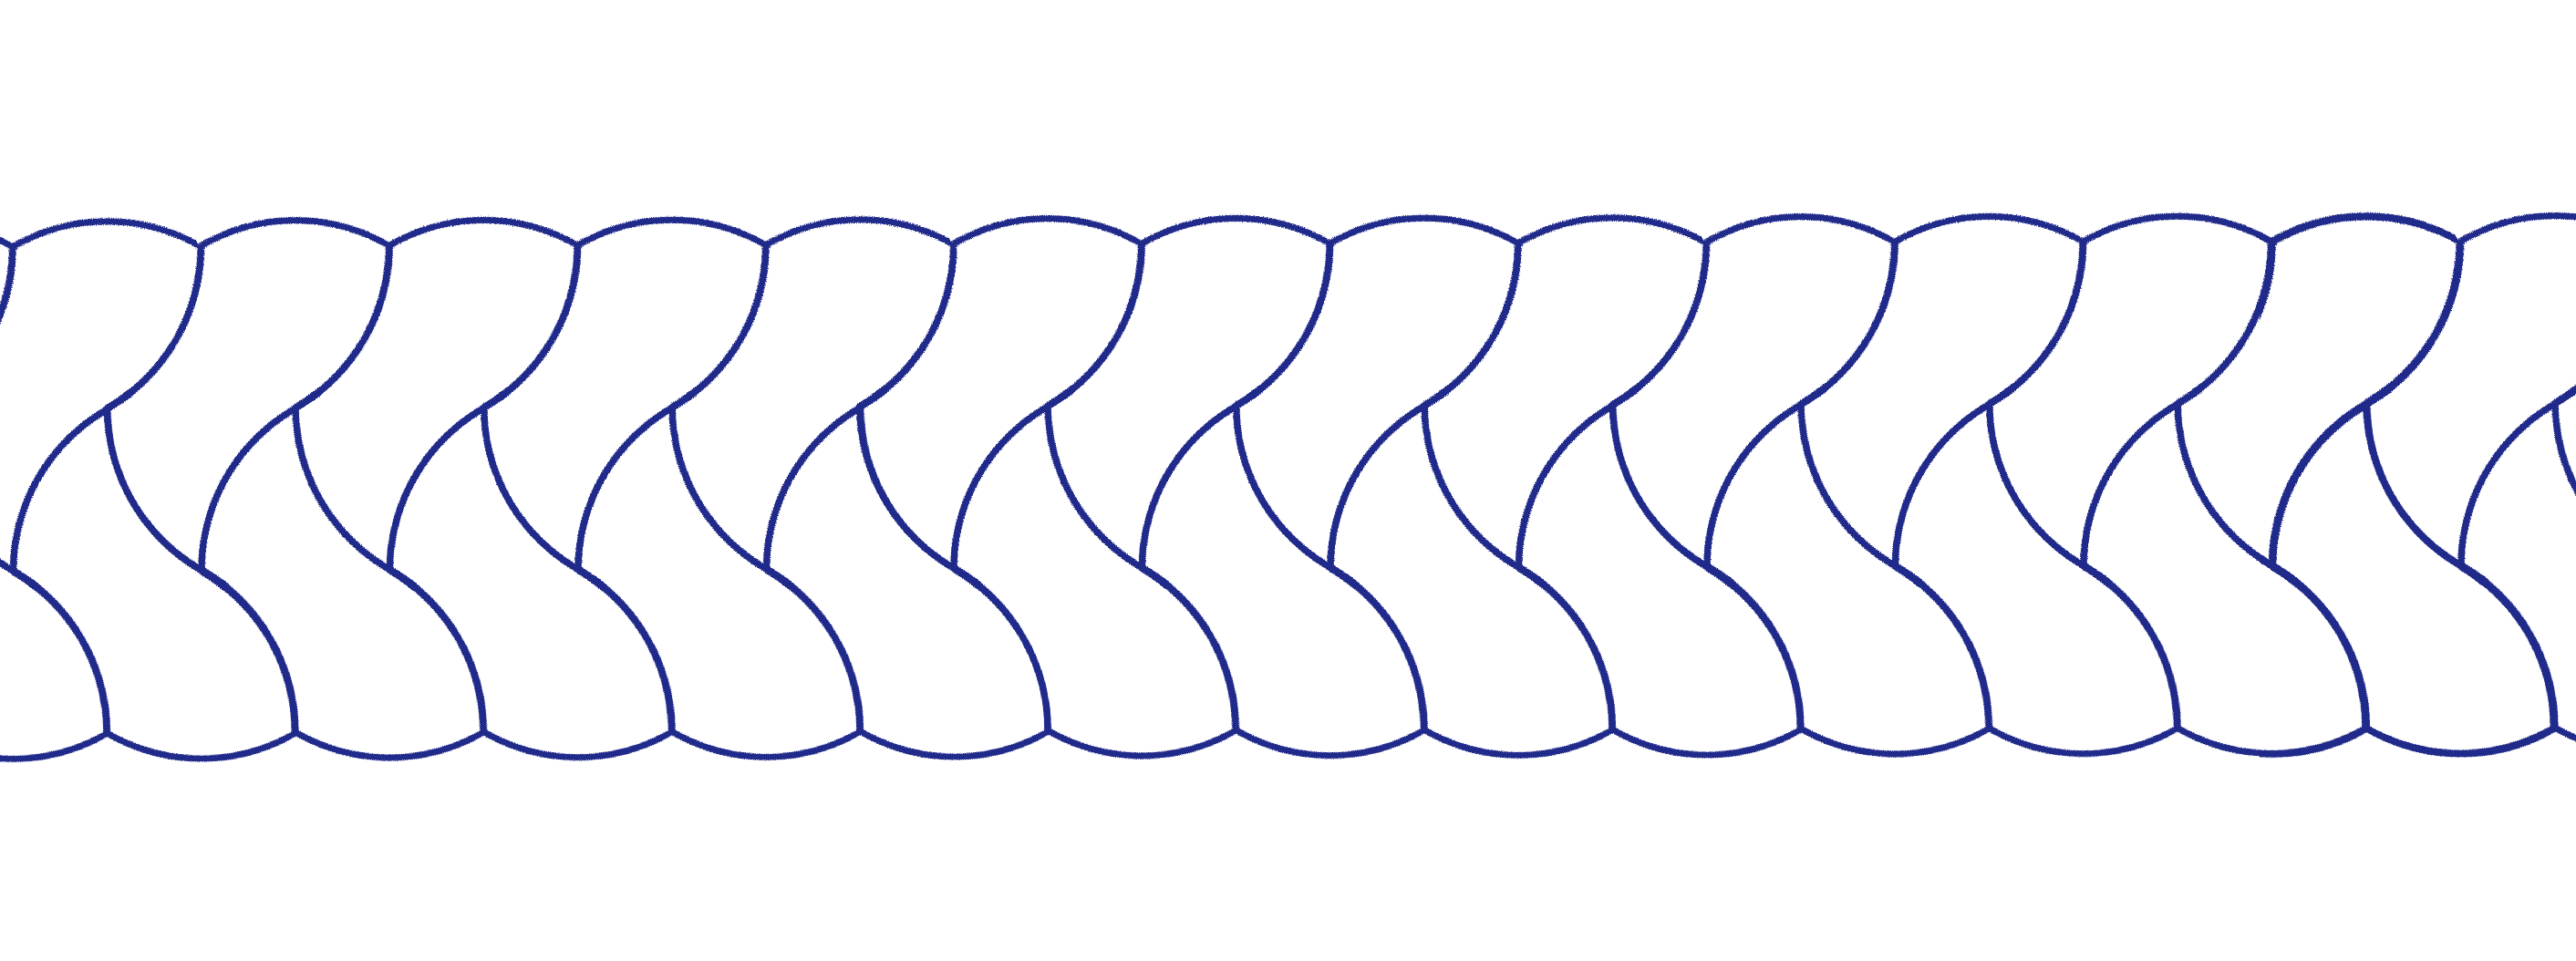
\includegraphics[width=12cm, trim = 0 2cm 0 2cm, clip]{pattern.png}
    \vspace{-0.3cm}
\end{figure}

    Each pentabend not on the ends now contributes a length of $\frac{\pi}{3}$ (one arc) to the perimeter, so it is easy to see that with a larger and larger shape, the roundness will approach $\frac{3}{\pi}.$
	
\end{document}